\section{Scaling Performance of $256^{3}$ problem}
Many authors in past have highlighted how bigger problems provide better scaling capabilities and our $256^{3}$ simulation fulfill such trend.
The medium sized problem shows better scaling performances compared to the small ones, although exhibit a slightly rugged behavior.
\par
\begin{figure}
\begin{center}
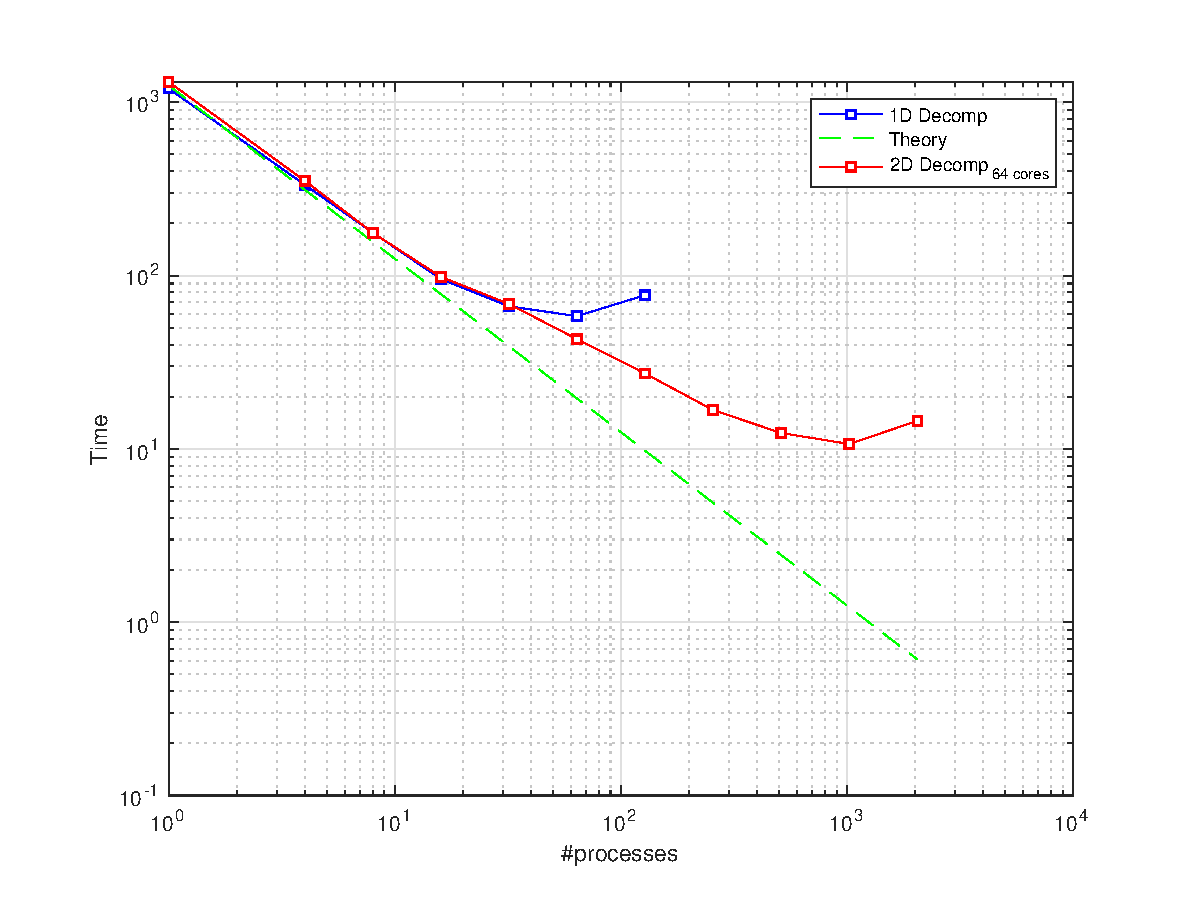
\includegraphics[scale=0.6]{grafici/1281}
\caption{Scaling performance of $256^{3}$ simulation}
\label{1281}
\end{center}
\end{figure}

\begin{figure}
\begin{center}
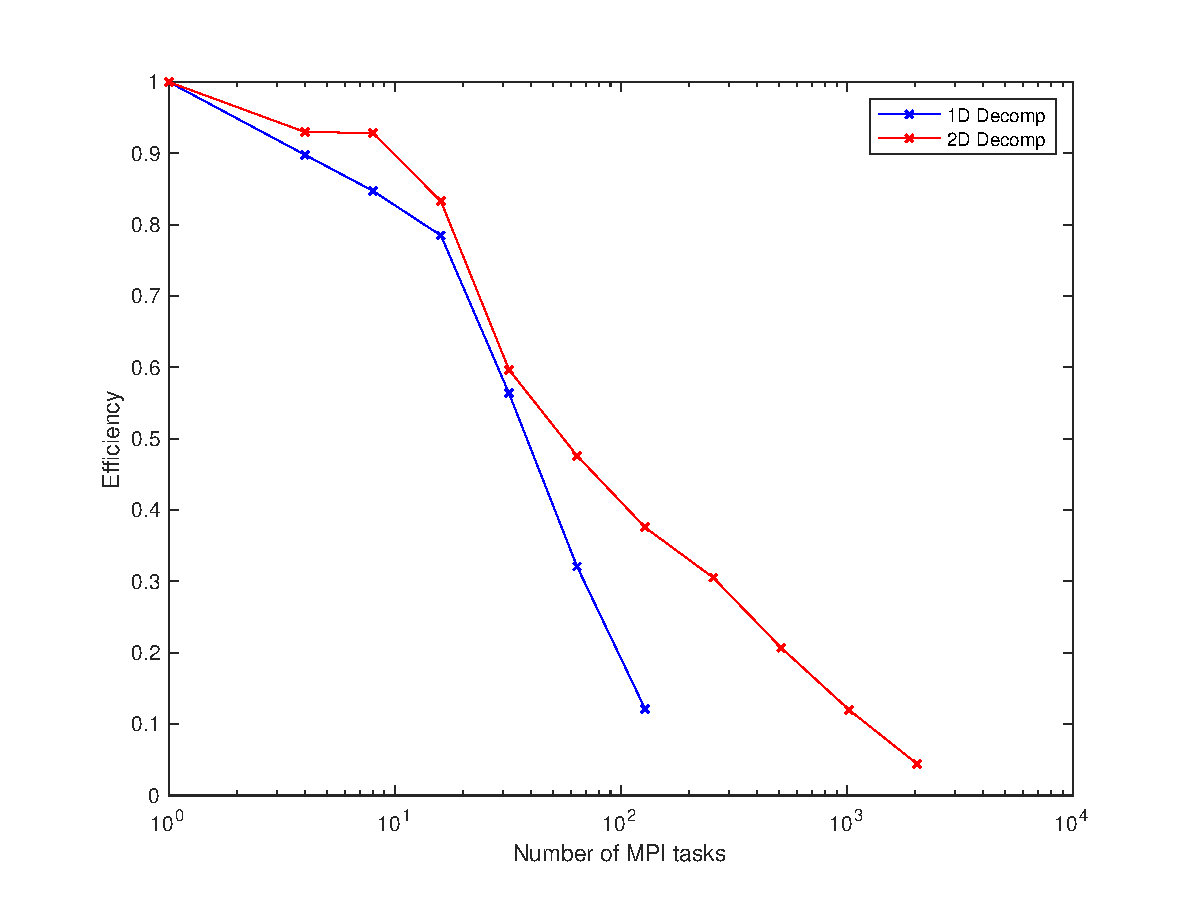
\includegraphics[scale=0.6]{grafici/1283}
\caption{Efficiency factor of $256^{3}$ simulation}
\label{1283}
\end{center}
\end{figure}

A slab decomposed algorithm provide gains of $\mathcal{O}(10)$ in terms of execution times, less than a pencil decomposed algorithm, but with better results for small processors grid. In fact, as depicted in figure~\ref{1281} the 1D decomposition curve achieve lower execution times than the 2D ones, until 32 cores.\\
Passed 32 cores the pencil decomposition prevails, reaching speedup factors above 120, with time savings in the order of magnitude of $\mathcal{O}(100)$ with respect to the single core runtime.
In the figure~\ref{1283} is possible to see the efficiencies achieved by the two methods, running on 64 threads per processor. It is important to denote the behavior of the pencil decomposed algorithm, which, until 8 cores are used, exhibits a very high scaling efficiency. \\
\par
Comparing image~\ref{1281} with its counterpart for the $128^{3}$ problem, figure~\ref{641} of page~\pageref{641}, we can see that the curves are quite similar. Both exhibits a very good fitting with the theoretical ones until 16 parallel processes take place. Once passed this threshold, the bigger problem maintains a better scaling efficiency, as we could see by comparing figure~\ref{1283} and~\ref{643}, for both decomposition methods. \par
The better efficiency allows to reach higher speedup factors at number of processes equality, and the larger dimensions move the performances peak towards higher number of threads, as is possible to see by looking at figure~\ref{1282}. The combination of this two factors doubles the last speedup factor, passing from 57, for the $128^{3}$ problem, to 122 for the $256^{3}$.\\

\begin{figure}
\begin{center}
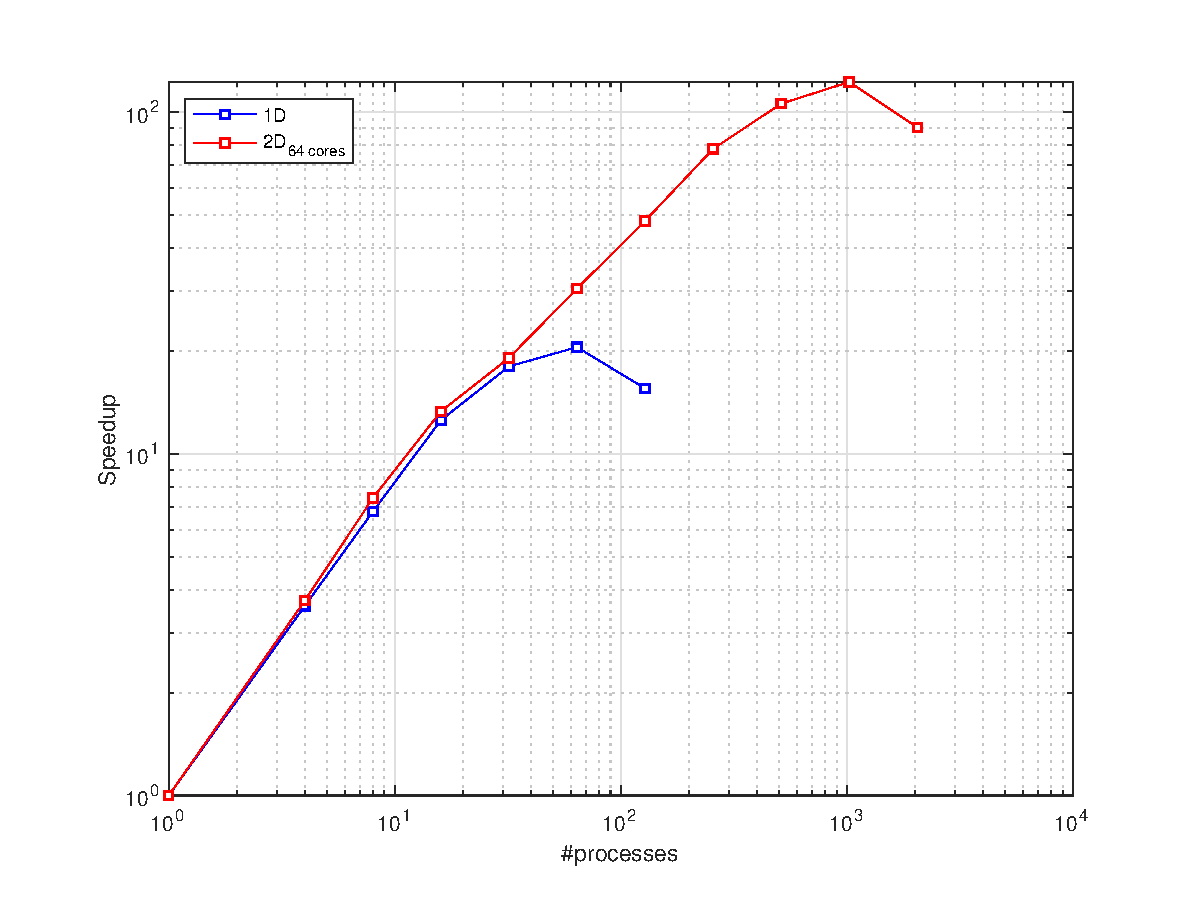
\includegraphics[scale=0.6]{grafici/1282}
\caption{Speedup performance factor of $256^{3}$ simulation}
\label{1282}
\end{center}
\end{figure}

\par
A comparison of the performances of 1D decomposition against the 2D for the present problem dimension is presented in table~\ref{128:data} of page~\pageref{128:data}.

\begin{table}
\caption{Data from $256^{3}$ simulation}
\begin{center}
\begin{tabular}{c c c c c}
\toprule
\textbf{\#Processes} & \textbf{Time [s]} & \textbf{Speedup} & \textbf{Efficiency [\%]} & \textbf{Decomp}\\
\midrule
\multirow{2}{*}{1} &  1198.8 & 1 & 100 & 1D\\
& 1309.7 & 14.28 & 89 & 2D\\
\hline
\multirow{2}{*}{4} &  333.7 & 3.59 & 90 & 1D\\
& 352.1 & 3.72 & 93 & 2D \\
\hline
\multirow{2}{*}{8} &  176.8 & 6.78 & 85 & 1D\\
& 176.3 & 7.43 & 93 & 2D\\
\hline
\multirow{2}{*}{16} & 95.5 & 12.56 & 78 & 1D\\
& 98.3 & 13.33 & 83 & 2D\\
\hline
\multirow{2}{*}{32} & 66.5 & 18.04 & 56.3 & 1D\\
& 68.6 & 19.1 & 60 & 2D\\
\hline
\multirow{2}{*}{64} & 58.4 & 20.54 & 32 & 1D\\
& 43 & 38.48 & 48 & 2D\\
\hline 
\multirow{2}{*}{128} & 77.1 & 15.55 & 12 & 1D\\
& 27.2 & 48.1 & 36 & 2D\\
\hline
256 & 16.8 & 78.19 & 31 & 2D\\
512 & 12.4 & 106.1 & 21 & 2D\\
1024 & 10.7 & 122.7 & 12 & 2D\\
2048 & 14.5 & 90.33 & 4 & 2D\\
\bottomrule
\end{tabular}
\end{center}
\label{128:data}
\end{table}


\par
Passed 8 cores, to recover high efficiency we must decrease the number of threads per processor. We have executed a detailed analysis varying the threads per processor number, seeking the optimization for both the decomposition methods.
\par
For what concern the slab decomposition the results, reported in table~\ref{128:data:1} on page~\pageref{128:data:1}, shows that, although slightly improvements have been achieved, the 1D decomposed algorithm is quite insensitive to cores per processor variations, showing constant speedups, efficiencies and timing.\\
\par 
\begin{figure}
\begin{center}
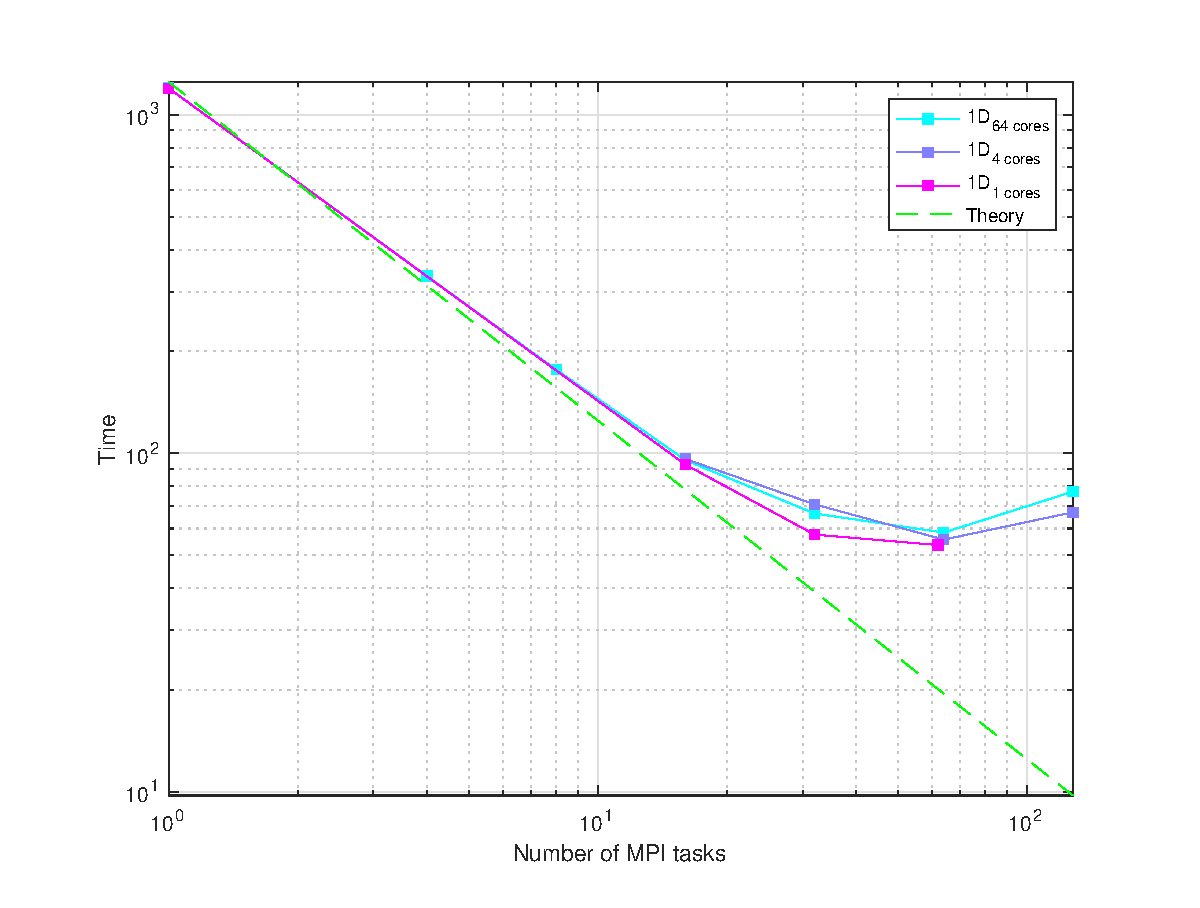
\includegraphics[scale=0.6]{grafici/1284}
\caption{Time scaling comparison using 1D decomposition for $256^{3}$ simulation}
\label{1284}
\end{center}
\end{figure}
\begin{figure}
\begin{center}
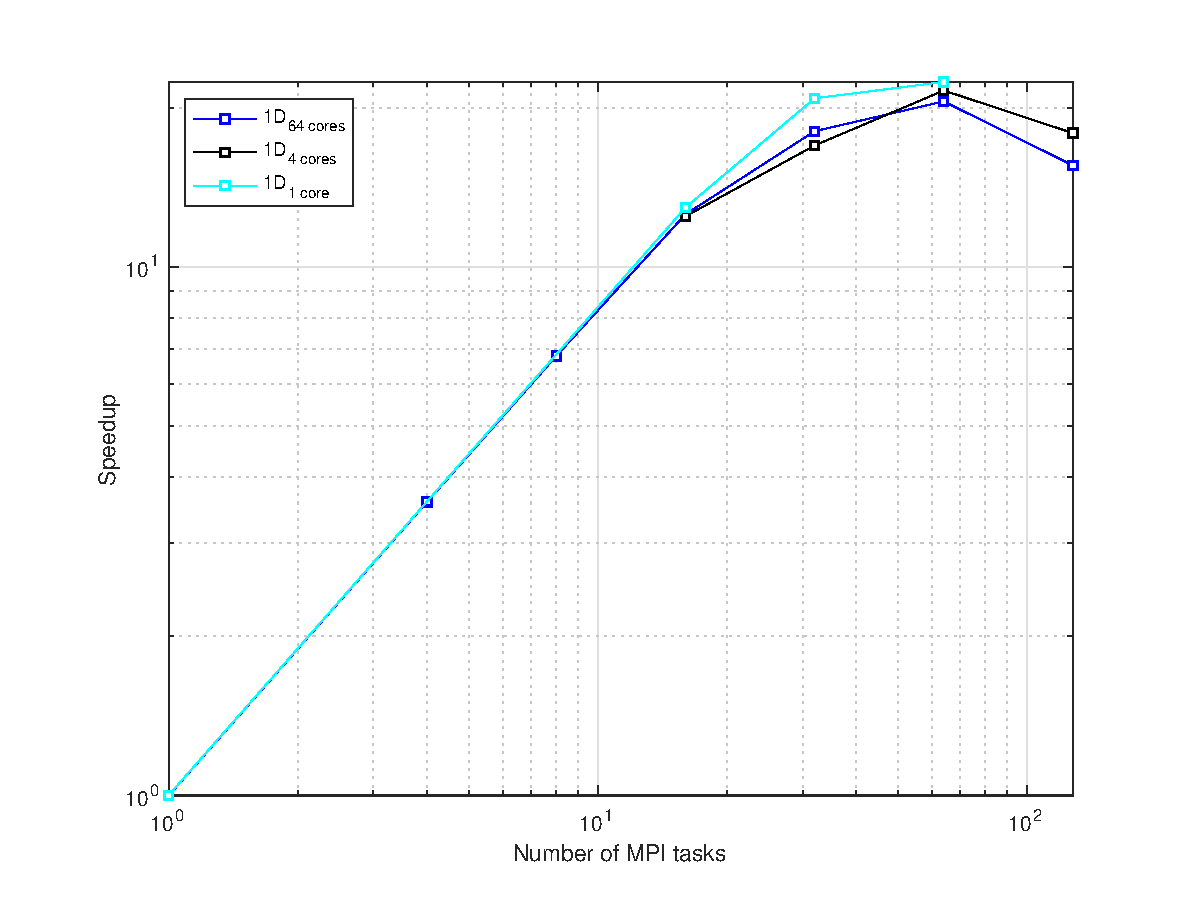
\includegraphics[scale=0.6]{grafici/1286}
\caption{Speedup comparison using 1D decomposition for $256^{3}$ simulation}
\label{1286}
\end{center}
\end{figure}
\begin{figure}
\begin{center}
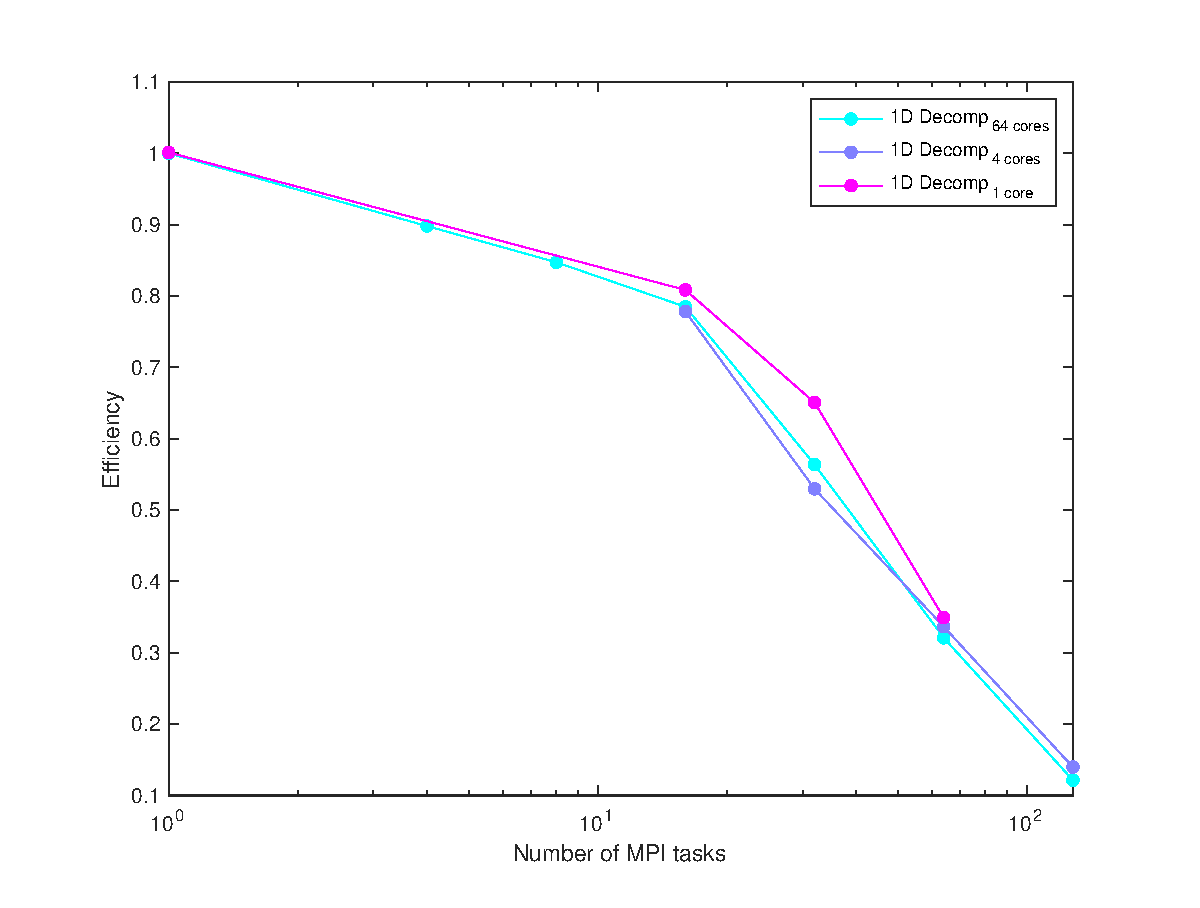
\includegraphics[scale=0.6]{grafici/1288}
\caption{Efficiency comparison using 1D decomposition for $256^{3}$ simulation}
\label{1288}
\end{center}
\end{figure}
Through figures~\ref{1284} and~\ref{1286} of page~\pageref{1284}, by looking at the single core curves, it is interesting to denote the presence of a knee, when 32 simultaneous processes take place, which origin a performances decrease. Such loss of linearity is present also using different cores per processor combinations, although on single core it appears to be more evident. Thus lead us to think that the intrinsic scaling limit, which depends on geometry and is caused by the raise in interprocessor communications time, has been reached. This limit clearly tear down the efficiency curve, as depicted in figure~\ref{1288}.\\

\begin{table}
\caption{Data from $256^{3}$ simulation, 1D decomposition}
\begin{center}
\begin{tabular}{c c c c c}
\toprule
\textbf{\#Processes} & \textbf{Time [s]} & \textbf{Speedup} & \textbf{Efficiency [\%]} & \textbf{cores}\\
\midrule
1 & 1198.75 & 1 & 100 & 64\\
4 &  333.7 & 3.59 & 90 & 64\\
8 &  176.8 & 6.78 & 85 & 64\\
\hline
\multirow{3}{*}{16} &  92.7 & 12.94 & 81 & 1\\
& 96.3 & 12.45 & 78 & 4\\
& 95.5 & 12.56 & 79 & 64\\
\hline
\multirow{3}{*}{32} &  57.6 & 20.82 & 65 & 1\\
& 70.7 & 16.95 & 53 & 4\\
& 66.5 & 18.04 & 56 & 64\\
\hline
\multirow{3}{*}{16} &  53.62 & 22.36 & 35 & 1\\
& 55.7 & 21.51 & 34 & 4\\
& 58.4 & 20.54 & 32 & 64\\
\bottomrule
\end{tabular}
\end{center}
\label{128:data:1}
\end{table}

\begin{table}
\caption{Data from $256^{3}$ simulation, 2D decomposition}
\begin{center}
\begin{tabular}{c c c c c}
\toprule
\textbf{\#Processes} & \textbf{Time [s]} & \textbf{Speedup} & \textbf{Efficiency [\%]} & \textbf{cores}\\
\midrule
1 & 1309.7 & 1 & 100 & 64 \\
4 & 352.1 & 3.72 & 93 & 64\\
8 & 176.3 & 7.43 & 93 & 64\\
16 & 98.3 & 13.33 & 83 & 64\\
\hline
\multirow{2}{*}{32} & 49.9 & 26.26 & 82 & 4\\
& 68.6 & 19.1 & 60 & 64\\
\hline
\multirow{2}{*}{64} & 29.3 & 44.73 & 70 & 4\\ 
 & 43 & 30.48 & 48 & 64\\
\hline
\multirow{4}{*}{128} & 21.4 & 61.17 &  48 & 4\\
& 21.5 & 61.03 & 48 & 8\\
& 23.2 & 56.58 & 44 & 32\\
& 27.2 & 48.1 & 38 & 64\\
\hline
\multirow{4}{*}{256} & 11.5 & 113.9 & 44 & 4\\
& 11.8 & 110.9 & 43 & 8\\
&13.5 & 97.23 & 38 & 32\\
&16.75 & 78.19 & 31 & 64\\
\hline
\multirow{4}{*}{512} & 9.4 & 140.1 & 27 & 4\\
&9.6 & 136.7 & 27 & 8\\
&11.8 & 110.7 & 22 & 32\\
&12.4 & 106.1 & 21 & 64\\
\hline
\multirow{3}{*}{1024} & 7.3 & 178.9 & 17 & 8\\
&9.9 & 132.7 & 13 & 32\\
&10.7 & 122.7 & 12 & 64\\
\hline
2048 & 14.5 & 90.33 & 4 & 64\\
\bottomrule
\end{tabular}
\end{center}
\label{128:data:2}
\end{table}

\par
Far more interesting is the pencil decomposed algorithm behavior. The data of such simulation, reported in table~\ref{128:data:2} of page~\pageref{128:data:2}, shows relevant improvements by varying the number of cores per processor. Another not yet cited, but always present tuning using 2D decomposition, is related to processor grid balancing. Our code provide optimal results when the processors grid have the same amount of MPI tasks among the two dimensions. Such behavior has been already described in deep in~\cite[39]{tesi:brach}. However it is not always possible to have the same number of threads in the two dimensions. In this case, after proper benchmark, we found that better results where achieved whether the number of tasks which decomposed the streamwise direction was lower than the other.
\par

\begin{figure}
\begin{center}
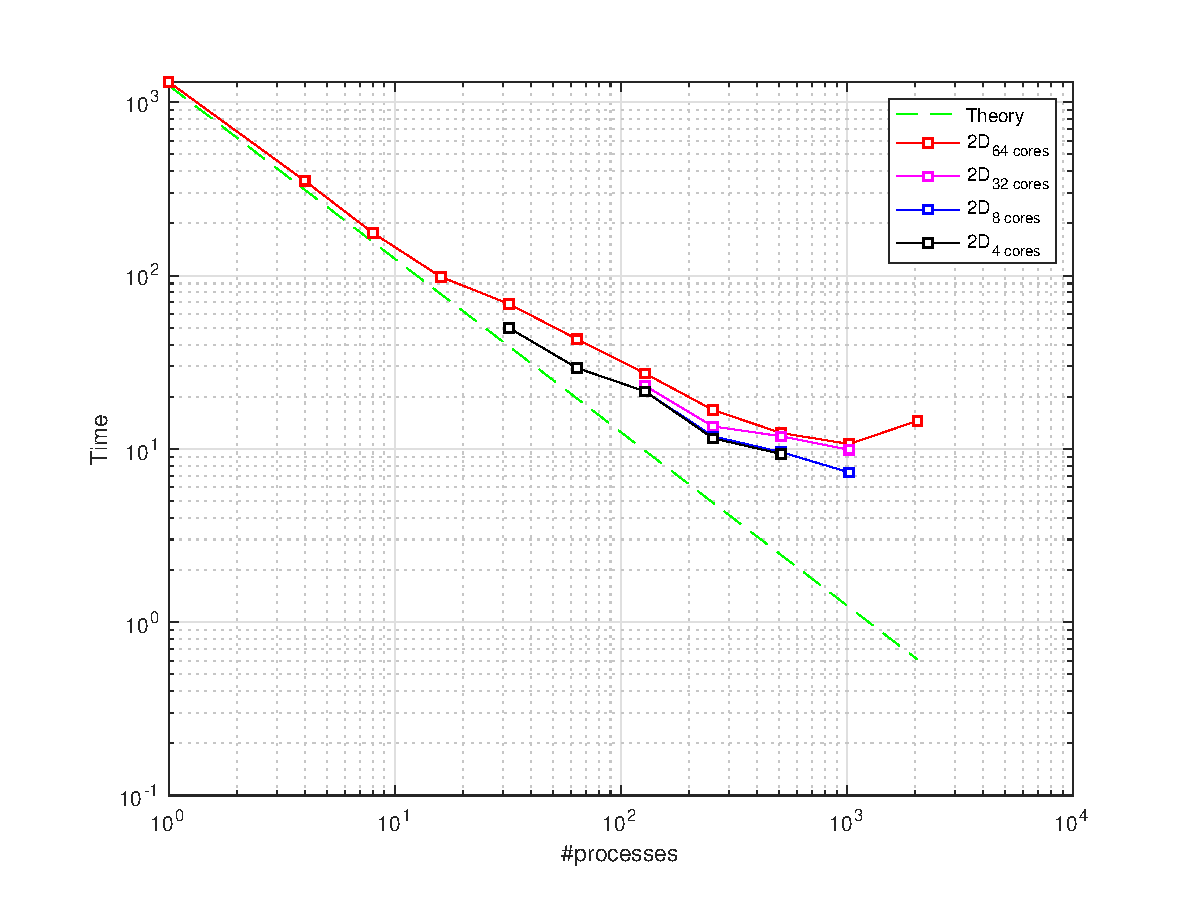
\includegraphics[scale=0.6]{grafici/1285}
\caption{Time scaling comparison using 2D decomposition for $256^{3}$ simulation}
\label{1285}
\end{center}
\end{figure}

As already said, the gains that we can obtain by reducing the number of threads per processor are high. 
Thus is due to the MPI standard that, although able to handle SMP processors~\cite{smp:processors}, lacks in efficiency as the number of cores becomes higher.
This is well highlighted by figure~\ref{1285}, in which we can see that a 4 cores approach can provide similar, or better, results than running the same code on 64 cores using twice the number of processes. The same reasoning holds also for an 8 versus 64 cores code execution. \par
This provide a boost in terms of execution time and, consequently, in terms of speedup factor, as can be recovered by looking at the results in table~\ref{128:data:2} where, at the peak, our speedup pass from 122.7 to 178.9.\par
The figure~\ref{1285} allow to see how, reducing the number of cores per processor, influence also the efficiency. Indeed we can see that running the code on 32 parallel processes using just 4 threads per nodes tends to realign the curve to the theoretical ones.\par
The efficiency curves can be seen in figure~\ref{1289}. They exhibit a rugged behavior with a marked trend to moves rightward as the number of cores per processor decreases.
For completeness the speedup factor curves has been reported, in figure~\ref{1287}.

\begin{figure}
\begin{center}
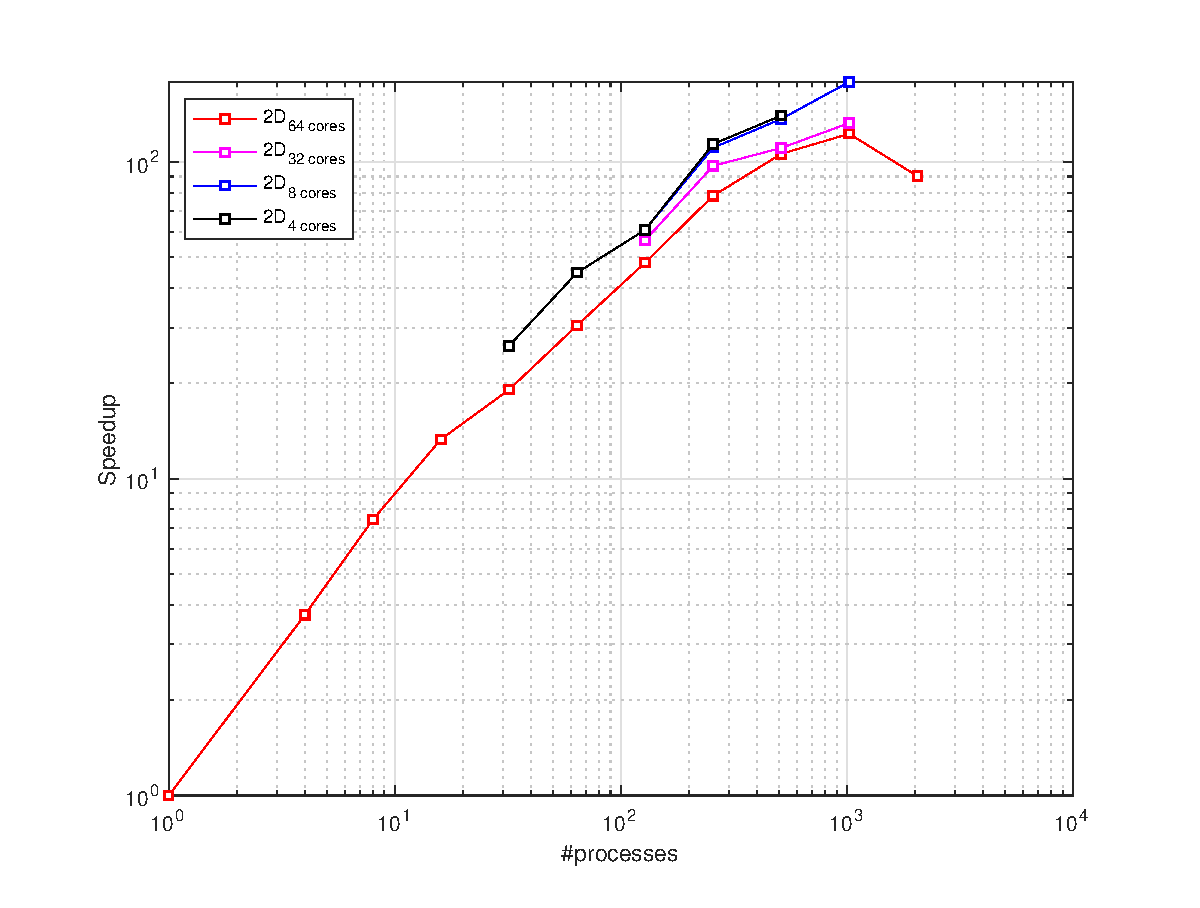
\includegraphics[scale=0.6]{grafici/1287}
\caption{Speedup comparison using 2D decomposition for $256^{3}$ simulation}
\label{1287}
\end{center}
\end{figure}

\begin{figure}
\begin{center}
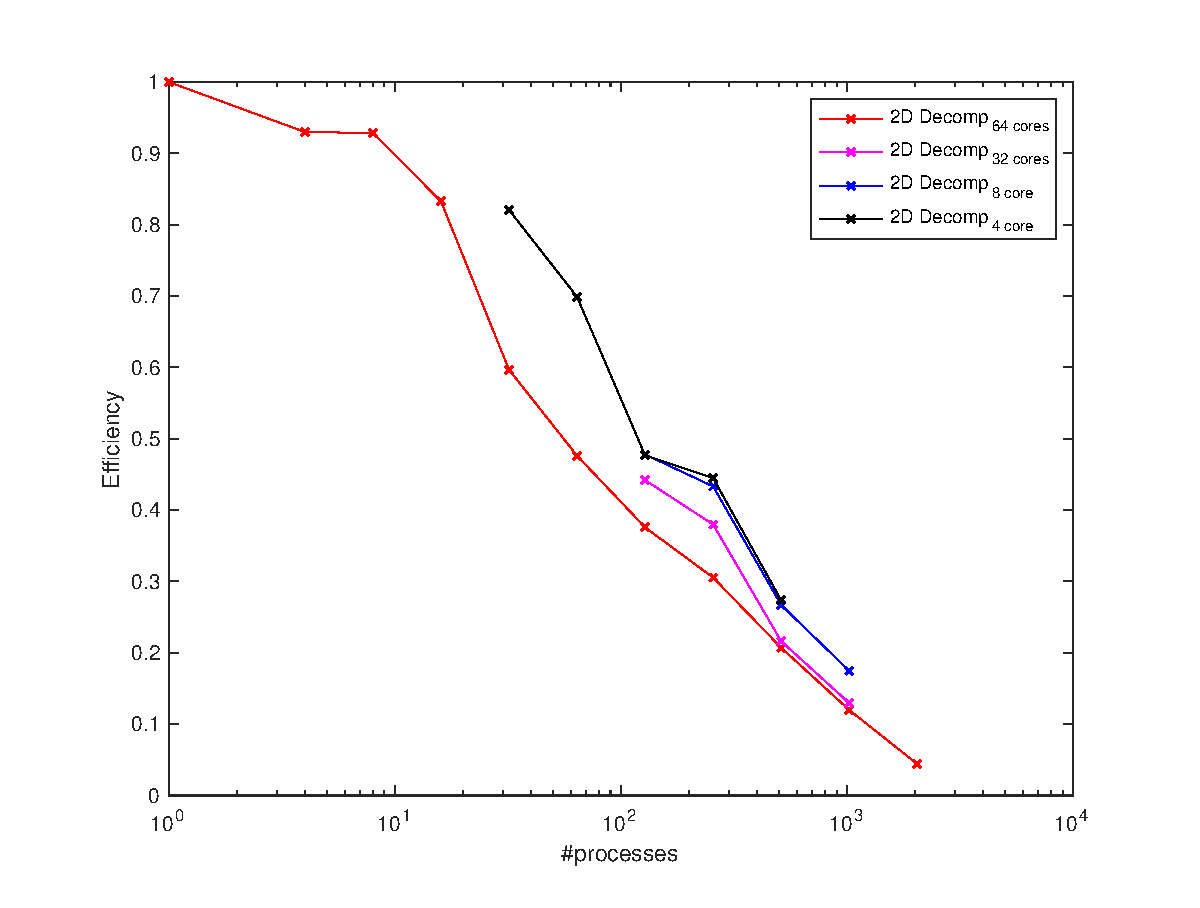
\includegraphics[scale=0.6]{grafici/1289}
\caption{Efficiency comparison using 2D decomposition for $256^{3}$ simulation}
\label{1289}
\end{center}
\end{figure}

